\documentclass[a4paper,oneside,12pt,final]{article}

\usepackage{fullpage}
\usepackage{graphicx}
\usepackage{booktabs}
\usepackage{paralist}
\usepackage{array}
\usepackage{enumitem}
\usepackage{rotating}
\usepackage{amsmath}

\setcounter{tocdepth}{1}

\title{\textsc{
\includegraphics[width=2cm]{./HAZ}\\\vspace{0.2cm}HAZ ENGINEERING\\Service Unit}\\\vspace{0.5cm}
\Large \textbf{Business Plan}}
\date{\today}
\author{}

\begin{document}


\maketitle
\normalsize

\newpage
\tableofcontents

\newpage

\section{General Description}

\textsc{HAZ Engineering} (also referred to as \emph{the Service Unit} hereafter) is a service provider to the contracting and manufacturing business units of HAZ Group, and serves and reports to HAZ Group Executive Committee (collectively referred to as \emph{HAZ Group} or \emph{the client} hereafter). The services provided by \textsc{HAZ Engineering} are design and engineering services. The function of the service unit shall be to act as a consultant engineer for the client's scope. The request for services for each project shall be initiated by request of the client. \\

The Service Unit base of operations will be located in Abu Dhabi, UAE; and will serve HAZ Group globally. The formation of this unit is to be considered a form of centralization of an already existing design service for contracted jobs and new tender bids, the aim of which is to achieve excellence of service by concentrating the required resources for this operation into one unit with a focused scope of work. The unit will have a dedicated head as Manager of the service unit, and will report to the HAZ Group Executive Committee.\\

\section{Services}

\subsection{Description of Services}

The scope of work for \textsc{HAZ Engineering} shall include the following:
\begin{enumerate}
	\item Project technical documents analysis and reporting in the context of the client's scope of work (\emph{i.e.} technical specifications, drawings\ldots{}etc.)
	\item Developing engineered solutions
	\item Structural analysis and documentation of calculation notes
	\item Design detailing
	\item Developing documented modeling (BIM, Parametric CAD\ldots{}etc.) methodologies to be adapted by the client's design team.
	\item Mock-up and prototype design
	\item Attending meetings for technical coordination purposes
\end{enumerate}

\subsection{Functional Benefits}

Engineering and design are core competencies for HAZ Group. The prime goal of the formation of \textsc{HAZ Engineering} Service Unit is the creation of a dedicated unit, capable of addressing the design needs of the contracting and manufacturing units with high efficiency and speed, under capable and specialized management.

\subsection{Stages of Development}
\label{sec:development}
\begin{enumerate}[label=\Alph*.]
	\item The formation of \textsc{HAZ Engineering} comes after recent developments in the group have resulted in the overloading of already existing business units which provide design and engineering services to the group (\emph{i.e.} HAZ Metal) without sufficient resources to cover the number and complexity of new tenders and/or contracted jobs. Accordingly, the first development to be achieved through \textsc{HAZ Engineering}, is to allocate dedicated resources, capable of handling design cases of higher complexity with greater efficiency using the already existing knowledge base and know-how of the group. This is to be considered the first stage of development of the service. 
	\item The next stage of development will be to actively add to the knowledge base of the group through basic Research and Development activities from within the service unit, which will help the unit adapt to new requirements and trends in the industry. Also, the liaison with other consultants and experts for jobs with high complexity and sophistication will be considered. These activities will be coordinated with HAZ Group Executive Committee, and should ultimately result in the formation of a separate dedicated Research and Development team.
\end{enumerate}
 
\section{Operational Procedures and Policies}
\subsection{Procedures}
\label{sec:procedures}
\begin{enumerate}
	\item A fully documented request (order) for a study case is presented by the client to \textsc{HAZ Engineering}, to include all relevant documentation, and description of requested work to be done.
	\item \textsc{HAZ Engineering} will initially review the client's request, and send a breakdown list of documents to be produced, and an expected time schedule, while also requesting any additional information that may be needed, for confirmation and feedback by the client.
	\item The documents are sent to the clients, allowing for any minor adjustments that may have resulted from misinterpretation of the information.
	\item The individual job will then be considered completed, and any further communication by the client with other parties concerning the completed job will not be the responsibility of \textsc{HAZ Engineering}.
\end{enumerate}

\subsection{Policies}
\begin{enumerate}
	\item If required; any coordination by \textsc{HAZ Engineering} with a third party shall be treated as a separate job, requiring a separate request by the client, with the same procedures as above (section \ref{sec:procedures}) being repeated.
	\item \textsc{HAZ Engineering} will not be responsible for follow up on the clients coordination or communication with a third party unless explicitly expressed in a formal request to \textsc{HAZ Engineering}.
	\item \textsc{HAZ Engineering} will not be responsible for bulk/mass production of shop drawings or models based on the proposed solutions of \textsc{HAZ Engineering}.
\end{enumerate}

\section{Management and Organization}

The organizational hierarchy will initially be flat, with only one level of management. The hierarchy will be subject to further restructuring in future revisions of this plan (refer to the Proposed Organization Chart in Figure \ref{fig:organization}).

\begin{figure}[h]
	\centering
	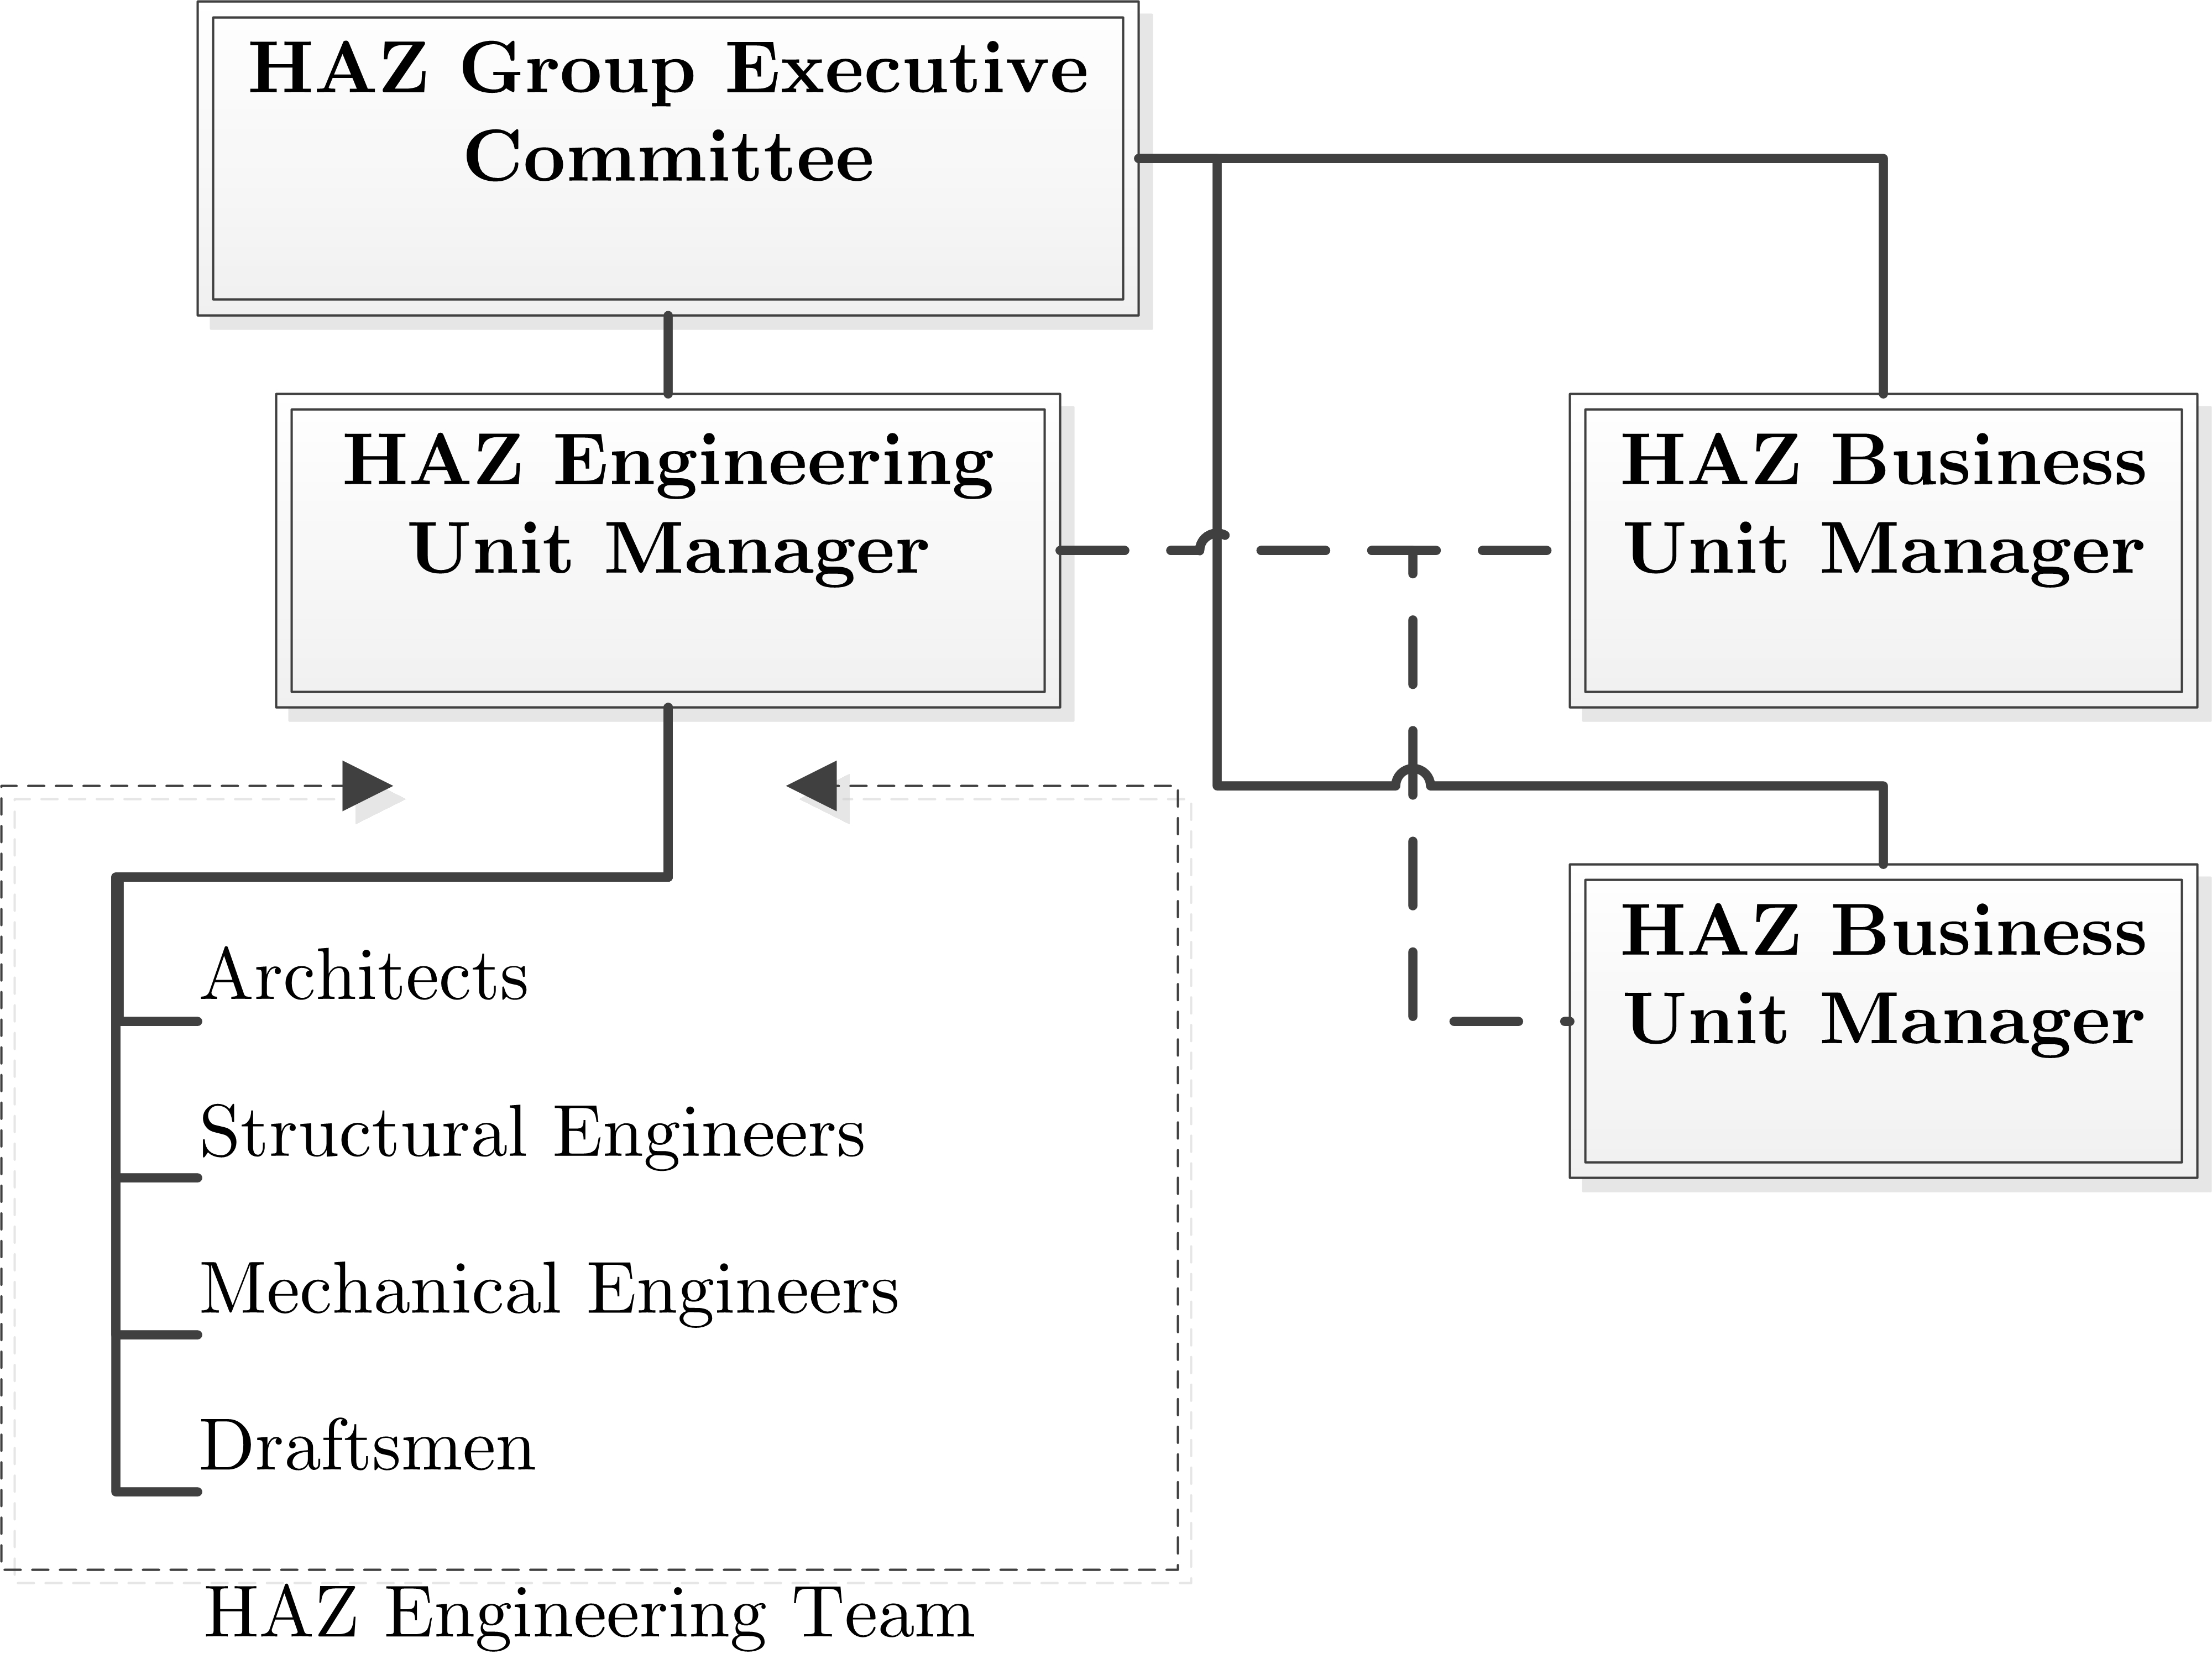
\includegraphics[width=8.5cm]{./organization}
	\caption{Proposed Organization Chart}
	\label{fig:organization}
\end{figure}

\subsection{Human Resources Plan}
\subsubsection{Grading and Recruitment}
\label{sec:grading}
\begin{enumerate}[label=\alph*.]
	\item Considering the proposed initial organization for \textsc{HAZ Engineering}; the grading process will be fairly simple, with only three levels:
	\begin{enumerate}[label=(1) ]
		\item \emph{Grade A}: for the Unit Manager position [21$\sim$24 points]; fully accountable for organization's work; works independently with broad policy, professional standards and budgetary limits; deals with highly complex assignments across the organization; regular contact with people at senior levels; develops and maintains relationships as a fundamental part of the job.
		\item \emph{Grade C}: for engineering positions [10$\sim$12 points]; works with moderate supervision; performs tasks requiring judgment and discretion; has knowledge of a variety of procedures, methods and techniques, has frequent contact with people inside his/her own working group and others within the organization 
		\item \emph{Grade D}: for the draftsmen position; [6 points]; works under close supervision; performs small number of routine tasks; has little or no contact with people outside of his/her own working group
	\end{enumerate}
	\item Detailed position requirements shall be provided separately, based on developments in the first two months. Nevertheless, the basic experience prerequisite for each position shall be as follows:
	\begin{enumerate}[label=(1)]
	\item \textbf{Architect}: minimum 3 years experience in the field of building and construction, with preference of experience in shop drawings production, and detailed coordination.
	\item \textbf{Structural Engineer}: minimum 3 years experience in the field of building and construction, with preference of experience in steel structures design.
	\item \textbf{Draftsman}: minimum 5$\sim$7 years experience in mechanical fixtures detailing.
	\end{enumerate}
	\item Anticipated Month of Initial Hiring shall be according to Table 1. Hirings needed after the first year will be determined in the first revised iteration of this business plan. All hirings are full-time contracts.
\end{enumerate}
	
\begin{table}[h]
	\centering
	\begin{tabular}{rccccc}
	\toprule
	\textbf{Month}&\textbf{1}&\textbf{2}&\textbf{3}&\textbf{4}&\textbf{5}\vspace{0.2cm}\\
	\midrule
	Manager&$\times$&&&&\\
	Architect&&&$\times$&&\\
	Structural Engineer&&&$\times$&\\
	Draftsman&&&&&$\times$\\
	\bottomrule
	\label{tab:MonthOfHiring}
	\end{tabular}
	\caption{Anticipated Month of Initial Hiring}
\end{table}

\subsubsection{Compensation and Benefits}

\begin{itemize}[label=\scriptsize$\bullet$]
	\item As all hirings will be full-time contracts; all employees will be entitled to full benefits. However, employee benefits such as transportation, medical cover/insurance\ldots{}etc., with the exception of various types of leaves (annual, sickness and emergency) shall be exchanged for an all-inclusive salary package.
	\item The salary/wage packages for each position as of the year 2015 shall be as per Table 2. Salary packages shall be subject to a 15\% yearly increment increase. Should the inflation rate as announced by the UAE government exceed 15\% in any given year; the incremental increase shall be adjusted accordingly. All salaries shall be paid in AED.
	\item Salaries are calculated using market \emph{median} wage average, as per statistical data collected from the UAE, for a specified range of years of experience for each job position. The data is also reinforced by a small-scale survey conducted with professionals in the UAE market, to validate the results.
	\item Incentives will be established through a bonus system. \textsc{HAZ Engineering} will be entitled to 10\% of any surplus from the annual balance sheet (refer to Section \ref{sec:finance} for the calculation method) to be divided and distributed by the unit Manager.
\end{itemize}

\begin{table}[h]
	\centering
	\begin{tabular}{rrr}
	\toprule
	\textbf{Position}&\textbf{Salary Package}&\textbf{Equivalent in USD}\\
	&\textbf{in AED}&\footnotesize AED:USD $=0.272$ \vspace{0.2cm}\\ 
	\midrule
	\normalsize
	Manager&32,000 AED&\$ 8,704 USD\\
	Architect&17,000 AED &\$ 4,624 USD\\
	Structural Engineer&17,000 AED &\$ 4,624 USD\\
	Draftsman&8,000 AED&\$ 2,176 USD\\
	\bottomrule
	\label{tab:wages}
	\end{tabular}
	\caption{Salary Packages (All-Inclusive)}
\end{table}

\subsubsection{Induction and Training}
A critical element of success of the unit; initial induction/orientation will be planned carefully to cover all relevant knowledge areas. Initial training will target the first development of the service (refer to section \ref{sec:development}), which will be coordinated with all concerned business units and current knowledge centers of the group.\\

The second phase of development will be achieved through active participation in any relevant events, conferences, expositions and training courses. The participation of representatives from \textsc{HAZ Engineering} will be coordinated with HAZ Executive Committee.
 
\section{Monitoring and Control}
\label{sec:control}

Performance assessment shall be made considering two performance elements \textbf{simultaneously}; the first being \emph{Critical Success Factors} (CSF), and the second being \emph{Key Performance Indicators} (KPI).\\

Critical Success Factors are external factors which have great impact on the performance and the success of the service unit to achieve its goals, which are representable to some extent in the KPI's. CSF's are not representable in numeral value, and are subject to subjective evaluation and judgment; nevertheless, they remain an indispensable tool for all-encompassing objective evaluation of the unit's performance.\\

Key Performance Indicators are represented numerically, and as monetary values, or time/duration values. These KPI's are a representation of the service unit's capability to achieve its \emph{targets}; which can be either performance based, such as average duration taken to complete a number of deliverables; and financial based, which will be discussed further in Section \ref{sec:finance}.

\subsection{Critical Success Factors}
\begin{enumerate}
	\item Retention of knowledge and experience; Employee Turnover Rate of 0\% for the first 3$\sim$5 years.
	\item Induction and initial training, and systematic development of knowledge and skills of all team members. Full cooperation of involved parties in the execution of the training program.
	\item The corporation's (HAZ Executive Committee) ability to coordinate the function of \textsc{HAZ Engineering} with other business units (the service unit does not implement a marketing strategy as functionally it serves HAZ Group internally; \emph{i.e.} implements a pull strategy); and reinforcing the strength of the service unit.
\end{enumerate}

\subsection{Key Performance Indicators}
\begin{enumerate}
	\item Number and \emph{value} (see section \ref{sec:finance}) of deliverables per month.
	\item Duration taken to complete a number of deliverables.
	\item Number and value of awarded projects, in which \textsc{HAZ Engineering} prepared its bidding technical documents (calculated as 1.5\% of the awarded contract value) .
\end{enumerate}

\section{Structure and Finance}
\label{sec:finance}

\subsection{Legal Form}
The service unit will be established in Abu Dhabi, UAE as a Limited Liability Company: ``\textsc{HAZ Engineering l.l.c.}'', with the local sponsor holding 100\% of the shares of the company. The company will be registered to the address of \textsc{HAZ Marble Industry and Trade l.l.c.} office in Abu Dhabi, UAE.

\subsection{Cost Center Performance Reports}
As a \emph{Cost Center}; financial performance of \textsc{HAZ Engineering} cannot be evaluated in simple terms of profitability as no actual revenue will be collected through account receivable transactions. Nevertheless, the establishment of a \emph{Managerial Accounting} system is necessary for performance analysis of the company, and to support management's planning and decision making process. This involves developing and maintaining a balance sheet of assets and liabilities, maintaining that no account receivables cash or cash eqivalent shall be collected.\\

Any \emph{financial} accounting services needed will be outsourced to \textsc{HAZ Marble Industry and Trade l.l.c.} for a predetermined fee (no actual cash transactions) to be included in the service unit's expenses.\\

\textsc{HAZ Engineering} will not claim any due monies from account receivables, and shall not be responsible for such collections to cover its expenses. All expenses of \textsc{HAZ Engineering} shall be covered by HAZ Group through its own chosen channels, with no responsibility on \textsc{HAZ Engineering} regarding the same.

\subsubsection{Expenses}
A summary of budgeted expenses for the first year of operation are shown in Table 3. Expenses shown are projected onto a schedule for an estimated cash out flow for the first year of operation (see section \ref{sec:cashflow}).

\begin{table}[h]
	\centering
	\begin{tabular}{p{4.1cm}p{5.5cm}rc}
	\toprule
	\textbf{Type}&\textbf{Description}&\textbf{Value}&Payable\\
	&&(AED)&Cash \vspace{0.2cm}\\ 
	\midrule
	\normalsize
	\textbf{Initial Expenses}&Company Establishment Fees&10,000&Yes\\
	&Acquisition of Equipment&50,000&\textsc{tbc}\\
	&Training Expenses&40,000&\textsc{tbc}\vspace{0.3cm}\\
	\textbf{Recurring Expenses}&Salaries&74,000&Yes\\
	\small (per month)\normalsize&Office Rental and Facilities&\textsc{tbc}&No\\
	\bottomrule
	\label{tab:expenses}
	\end{tabular}\vspace{-0.5cm}
	\caption{Expenses of First Year of Operation}
\end{table}

\subsubsection{Operating Income}

Services provided by \textsc{HAZ Engineering l.l.c.} shall be invoiced to the clients on a deliverable and man-hour basis. The cost of service shall be determined by a minimum (per deliverable) and controlled for increase through a calculation of man-hours, should the job require exceptional allocation of resources.\\

The balance sheet surplus ($=\text{invoiced value} -\text{expenses}$) will be considered an \emph{Operating Income}, and shall be the basis for evaluation of profitability of the company as a cost center, and for bonus calculation.

Pricing of services is shown in Table 4. Man-hour rates are hourly, and have been calculated for the three grades as shown in section \ref{sec:grading}.

\begin{table}[h]
	\centering
	\begin{tabular}{lllll}
	\toprule
	\textbf{Deliverable}&\textbf{Base Price}&\textbf{Grade A}&\textbf{Grade C}&\textbf{Grade D}\\
	&\footnotesize AED&\footnotesize AED/hour&\footnotesize AED/hour&\footnotesize AED/hour \vspace{0.2cm}\\ 
	\midrule
	\normalsize
	Contractual Document Analysis&4,000&332&133&\textsc{n/a}\\
	Calculation Note\footnotesize/per item&3,500&249&223&\textsc{n/a}\\
	Design Detail\footnotesize/per item&1,000&332&178&84\\
	Method Statement&4,000&350&178&\textsc{n/a}\\
	Prototype Design&5,500&350&249&84\\
	Visits \footnotesize (excluding expenses)&\textsc{n/a}&332&249&\textsc{n/a}\\
	\bottomrule
	\label{tab:serviceprice}
	\end{tabular}
	\caption{Service Pricing}
\end{table}

\newpage
\subsubsection{Cash Out Flow}
\label{sec:cashflow}

\begin{table}[h]
	\centering
	\begin{tabular}{lrrr}
	\toprule
	\textbf{Month}&\textbf{Expenses}&\textbf{Balance}&\textbf{Balance}\\ 
	&\footnotesize{AED}&\footnotesize{AED}&\footnotesize{($\times{}0.272$)} USD\vspace{0.2cm}\\ 
	\midrule
	\normalsize
	1&47,000 &-- 47,000&(--\$12,784)\\
	2&32,000 &-- 79,000&(--\$21,488)\\
	3&111,000 &-- 190,000&(--\$51,680)\\
	4&106,000 &-- 296,000&(--\$80,512)\\
	5&74,000 &-- 370,000&(--\$100,640)\\
	6&74,000 &-- 444,000&(--\$120,768)\\
	7&74,000 &-- 518,000&(--\$157,760)\\
	8&74,000 &-- 592,000&(--\$161,024)\\
	9&74,000 &-- 666,000&(--\$181,152)\\
	10&74,000 &-- 740,000&(--\$201,280)\\
	11&74,000 &-- 814,000&(--\$221,408)\\
	12&74,000 &-- 888,000&(--\$241,536)\\
	\midrule
	&1\textsuperscript{st} Year Expenses&\textbf{888,000 AED}&(\$241,536 USD)\\
	&Budget&&\\
	\bottomrule
	\label{tab:cashflow}
	\end{tabular}
	\caption{Cash Out Flow for the First Year of Operation}
\end{table}

\begin{figure}[h!]
	\centering
	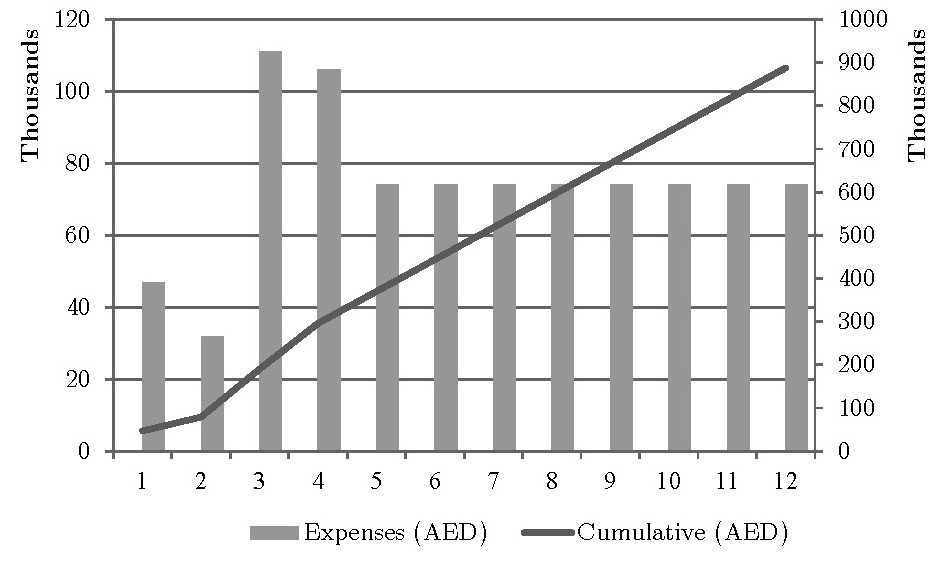
\includegraphics[width=0.75\textwidth]{./Histogram}
	\caption{Cash Out Flow Histogarm and S-Curve}
	\label{fig:histogram}
\end{figure}

\end{document}